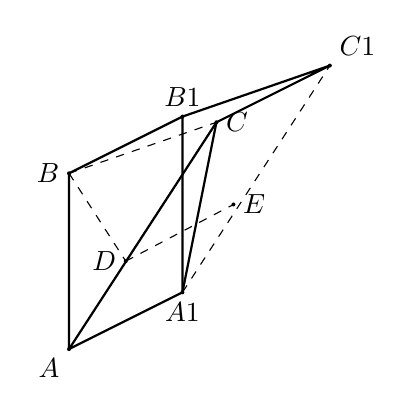
\begin{tikzpicture}[scale=.72,>=stealth]
\coordinate (A) at (0,0); \coordinate (B) at (0,3.1);
\coordinate (C) at (2.6,4.0); \coordinate (A1) at (2.0,1.0);
\coordinate (B1) at (2.0,4.1); \coordinate (C1) at (4.6,5.0);
\coordinate (D) at (1.0,1.55); \coordinate (E) at (2.9,2.55);
\draw[thick] (A)--(B)--(B1)--(A1)--cycle;
\draw[thick] (B1)--(C1)--(C)--(A);
\draw[dashed] (A)--(A1) (B)--(C) (A1)--(C1);
\draw[dashed] (D)--(E) (B)--(D)--(C);
\draw[thick] (A1)--(C);
\foreach \p/\pos in {A/below left,B/left,C/right,A1/below,B1/above,C1/above right,D/left,E/right}
  {\fill (\p) circle (1pt) node[\pos] {$\p$};}
\end{tikzpicture}
